\documentclass[12pt]{article}
\usepackage[utf8]{inputenc}
\usepackage{graphicx} % This package is used to render figures
\usepackage{booktabs} % This package is used to make tables look nice
\usepackage{tikz}  % This package can be used to make graphs (i.e., nodes with edges)
\usepackage{parskip}
\usepackage{algorithm} % This package is used to render algorithms
\usepackage{amsmath} % These packages are for math symbols
\usepackage{amsfonts}
\usepackage{amssymb}

\usepackage[noend]{algpseudocode}
\usepackage{url}

\graphicspath{{./figures}} % This is where you find the figures

\usepackage{times}
\usepackage{helvet}
\usepackage{courier}
\usepackage{listings}


% The file iccc.sty is the style file for ICCC proceedings.
%

\lstdefinestyle{mystyle}{
    language=Python,
    basicstyle=\ttfamily,
    keywordstyle=\color{blue},
    commentstyle=\color{green!50!black},
    stringstyle=\color{red},
    showstringspaces=false,
    numbers=left,
    numberstyle=\normalfont,
    numbersep=5pt,
    breaklines=true,
    breakatwhitespace=true,
    tabsize=2,
    captionpos=b
}


\title{Report on Networking Routing}
\author{Sabal Subedi \\
Master's in Computer Science\\
Idaho State University\\
Pocatello, ID, 83209  USA\\
sabalsubedi@isu.edu\\
}               


\begin{document}

\maketitle

\begin{abstract}
This project report summarizes the use of the  Dijkstra’s algorithm to find paths through a graph representing a network routing problem.
\end{abstract}
    
\section{Introduction}
Dijkstra's algorithm is widely used algorithm in graph theory for finding the shortest path between nodes in a graph with non-negative edge weights.\\
Dijkstra's algorithm relies heavily on the use of a priority queue to efficiently select the next node to visit during the exploration of the graph. The priority queue is used to keep track of the nodes that are candidates for visiting, with the priority being determined by the tentative distance from the start node. \\
I will use two of such priority queue: array and binary heap, to analyze the Asymptotic notation of Dijkstra’s algorithm.

\newpage
\section{Pseudocode and Asymptotic Analysis}

\subsection{Pseudocode for unsorted array priority queue}
\begin{lstlisting}[style=mystyle]
    def dijkstra_implementataion(self, srcIndex, use_heap=False):
        pq = object of array queue if not use_heap else object of binary heap queue
        # initializing the prev array to nil
        self.prev_array = [None] * len(self.network.nodes)

        # Start with the source node and updating the dist value to 0
        pq.insert(srcIndex)
        pq.decrease_key(0, srcIndex)

        # iterate until there is node in queue
        while pq.queue:
            curr_min_node_index = pq.delete_min()
            curr_node = self.network.nodes[curr_min_node_index]

            # Check each edge from the lowest distance node
            for edge in curr_node.neighbors:
                node_index = edge.dest.node_id
                new_distance = pq.dist[curr_min_node_index] + edge.length
                if new_distance < pq.dist[node_index]:
                    pq.insert(node_index)
                    self.prev_array[node_index] = curr_min_node_index
                    pq.decrease_key(new_distance, node_index)
    \end{lstlisting}

\newpage

\noindent\textbf{Time complexity and space complexity} \\
\textbf{Using unsorted Array}
\begin{enumerate}
    \item insert method takes $O(1)$ time and $O(1)$ space; this method appends new node to the queue
    \item decrease\_key method takes $O(1)$ time and $O(1)$ space; this method updates the distance of node 
    \item delete\_min method takes $O(n)$ times and $O(1)$ space; this method scans the queue and return the the node with minimum distance value
\end{enumerate}
\begin{equation} % You should use descriptive variable names (not eq1)
\begin{split}
    &Time\_complexity = O(1) + O(1) + O(n) * ( O(1) + O(n)) \approx O(n^2) \approx O(|V|^2) \\
    &Space\_complexity = O(n) \approx O(|V|) \\
    &where,\ V \ is \ verticies \ in \ graph
\end{split}
\end{equation}

\textbf{Using binary heap}
\begin{enumerate}
    \item insert method takes $O(\log n)$ time and $O(1)$ space; this method appends new node to the queue
    \item decrease\_key method has two function calls \\ 
    bubble\_up takes $O(\log n)$ times; this method switch the parent and child node in a tree of depth $O(\log n)$ \\
    swap\_nodes takes $O(1)$ time \\
    and space complexity is $O(1)$ space
    \item delete\_min method has two function calls \\
    bubble\_down takes $O(\log n)$ times; this method switch the root and child node in a tree of depth $O(\log n)$\\
    swap\_nodes takes $O(1)$ time\\
    space complexity is $O(1)$ space 
\end{enumerate}
\begin{equation} % You should use descriptive variable names (not eq1)
\begin{split}
    &Time\_complexity = O(1) + O(\log n) + O(n) * (O(\log n) + O(\log n)) \approx O(n \log n) \approx O(|V| \log |V|) \\
    &Space\_complexity = O(n) \approx O(|V|) \\
    &where,\ V \ is \ verticies \ in \ graph
\end{split}
\end{equation}

\subsection{Pseudocode for unsorted array priority queue}
\begin{lstlisting}[style=mystyle]
    class ArrayPriorityQueue:
        def __init__(self, nodes):
            # initializing the dist array to infinite
            self.dist = [math.inf] * len(nodes)
            self.queue = []

        # adds new item in queue
        def insert(self, node_index):
            self.queue.append(node_index)
    
        # updates the distance value of a node
        def decrease_key(self, dist, node_index):
            self.dist[node_index] = dist
        
        # finds a node with minimum distance and return it after removing it from the queue
        def delete_min(self):
            if not self.queue:
                return None
    
            min_node = None
            min_distance = math.inf
    
            for node in self.queue:
                if self.dist[node] < min_distance:
                    min_node = node
                    min_distance = self.dist[node]
    
            self.queue.remove(min_node)
            return min_node
    \end{lstlisting}

\newpage

\noindent\textbf{Time complexity and space complexity} \\
\begin{enumerate}
    \item initialization takes $O(1)$ times to initialize the dist, and queue,\\
     and $O(n)$ space to store the dist, and queue
    \item insert method takes $O(1)$ time and $O(1)$ space
    \item decrease\_key method takes $O(1)$ time and $O(1)$ space 
    \item delete\_min method takes $O(n)$ times and $O(1)$ space 
\end{enumerate}
\begin{equation} % You should use descriptive variable names (not eq1)
\begin{split}
    &Time\_complexity = O(1) + O(1) + O(1) + O(n) \approx O(n) \approx O(|V|) \\
    &Space\_complexity = O(n) + O(1) + O(1) + O(1) \approx O(n) \approx O(|V|) \\
    &where,\ V \ is \ verticies \ in \ graph
\end{split}
\end{equation}


\subsection{Pseudocode for binary heap priority queue}
\begin{lstlisting}[style=mystyle]
    class HeapPriorityQueue:
    def __init__(self, nodes):
        # initializing the distance to infinity
        self.dist = [math.inf] * len(nodes)
        self.queue = []
        # initializing the pointer of the tree to infinity
        self.q_pointer = [math.inf] * len(nodes)

    # add a node into the heap
    def insert(self, node_index):
        self.queue.append(node_index)
        self.q_pointer[node_index] = len(self.queue) - 1
        self.bubble_up(len(self.queue) - 1)

    # adjust the distance update of nodes
    def decrease_key(self, dist, node_index):
        self.dist[node_index] = dist
        self.bubble_up(self.q_pointer[node_index])

    # bubble_up maintains the property of heap after insertion or decrease key operation
    def bubble_up(self, child_index):
        while child_index > 0:
            parent_index = (child_index - 1) // 2
            if (
                self.dist[self.queue[child_index]]
                >= self.dist[self.queue[parent_index]]
            ):
                break
            self.swap_nodes(child_index, parent_index)
            child_index = parent_index

    # return the minimum element from the heap and removes it
    def delete_min(self):
        if not self.queue:
            return None

        min_index = self.queue[0]
        if len(self.queue) == 1:
            self.queue.pop()
            return min_index

        last_index = len(self.queue) - 1
        self.swap_nodes(0, last_index)
        self.queue.pop() # swaps the item at the end with root and return the root node
        self.bubble_down(0)

        return min_index

    # restores the heap property starting from the given parent_index
    def bubble_down(self, parent_index):
    while True:
        left_child_index = 2 * parent_index + 1
        if left_child_index >= len(self.queue):
            break

        child_index_left = left_child_index
        child_index_right = left_child_index + 1
        if (
            child_index_right < len(self.queue)
            and self.dist[self.queue[child_index_right]]
            < self.dist[self.queue[left_child_index]]
        ):
            child_index_left = child_index_right

        # checking the distance of parent node and the smallest child node
        if (
            self.dist[self.queue[parent_index]]
            <= self.dist[self.queue[child_index_left]]
        ):
            break

        self.swap_nodes(parent_index, child_index_left)
        parent_index = child_index_left

    # perform the swap between nodes
    def swap_nodes(self, i, j):
        self.queue[i], self.queue[j] = self.queue[j], self.queue[i]
        self.q_pointer[self.queue[i]] = i
        self.q_pointer[self.queue[j]] = j
    \end{lstlisting}

\newpage
\noindent\textbf{Time complexity and space complexity} \\
\begin{enumerate}
    \item initialization takes $O(1)$ times to create the dist, queue, and pointer, \\
    and $O(n)$ space to store the dist, queue, and pointer
    \item insert method takes $O(\log n)$ time and $O(1)$ space
    \item decrease\_key method has two function calls \\
    bubble\_up takes $O(\log n)$ times \\
    swap\_nodes takes $O(1)$ time \\
    and space complexity is $O(1)$ space
    \item delete\_min method has two function calls \\
    bubble\_down takes $O(\log n)$ times\\
    swap\_nodes takes $O(1)$ time\\
    space complexity is $O(1)$ space 
\end{enumerate}
\begin{equation} % You should use descriptive variable names (not eq1)
\begin{split}
    &Time\_complexity = O(1) + O(\log n) + O(\log n) + O(\log n) \approx O(\log n) \approx O(\log |V|) \\
    &Space\_complexity = O(n) + O(1) + O(1) + O(1) + O(1) \approx O(n) \approx O(|V|) \\
    &where,\ V \ is \ verticies \ in \ graph
\end{split}
\end{equation}

\newpage

\section{Observations and Results}

\subsection{Observation Table}
\begin{table}[h]
    \centering
    \begin{tabular}{|c|c|c|c|c|c|c|c|}
    \hline
    Queue Type & Size & 1 & 2 & 3 & 4 & 5 & Mean time\\
    \hline
    Array       & 100       & 0.0000    & 0.0000    & 0.0000    & 0.0000    & 0.0010    & 0.0002\\
    Array       & 1000      & 0.0109    & 0.0096    & 0.0119    & 0.0095    & 0.0101    & 0.0104\\
    Array       & 10000     & 0.9208    & 1.1623    & 1.2870    & 1.2569    & 1.1836    & 1.1621\\
    Array       & 100000    & 135.5281  & 122.2875  & 141.2688  & 165.9068  & 130.2860  & 139.0554\\ 
    \hline
    Binary Heap       & 100       & 0.0000    & 0.0010    & 0.0000    & 0.0010    & 0.0000   & 0.0002\\
    Binary Heap       & 1000      & 0.0050    & 0.0050    & 0.0045    & 0.0055    & 0.0051   & 0.0050\\
    Binary Heap       & 10000     & 0.0738    & 0.0951    & 1.1093    & 0.1054    & 1.1090   & 0.4985\\
    Binary Heap       & 100000    & 1.1646    & 1.0881    & 1.3380    & 1.1206    & 1.1153   & 1.1652\\ 
    Binary Heap       & 1000000   & 21.2837   & 20.0075   & 20.0632   & 20.4115   & 20.2848  & 20.4101\\ 
    \hline
    \end{tabular}
\caption{Time taken to run Dijkstra’s Algorithm in different priority queue}
\label{tab:arraycoltable}
\end{table}

\noindent The table (in Table 1) shows different time taken to run the different sample size with random seed, source and target. Observing the obtained data, I can estimate the time needed to compute the tree using array with size 1000000. The time taken by the array is growing at a rate of $10^2$.\\
To estimate the run time of Array for size 1000000, I can use the average time taken by array queue to get the tree for size 100000 using following formula,\\
\begin{equation*} % You should use descriptive variable names (not eq1)
    \begin{split}
        Array\ queue\ of\ size\ 1000000 & = ((1000000/100000)^2) * avg\ time\ for\ array\ of\ size\ 100000  \\
        & = 100 * 139.0554\\
        & = 13905.544 \ sec \\
    \end{split}
\end{equation*}


\newpage

\begin{figure}[h]. % the 't' asks LaTeX to put this figure on the top of the page   
    \begin{center}
      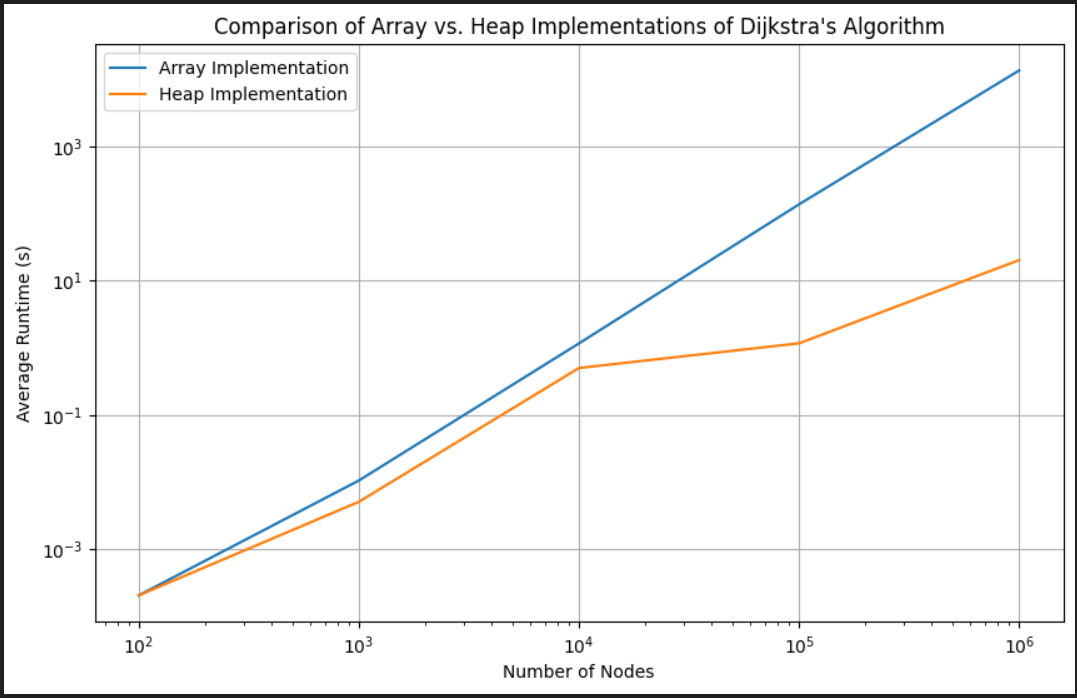
\includegraphics[width=0.80\linewidth]{figures/plot.png} 
      \caption{Plot between the different sample sizes and the time taken by the project}\label{fig:plot}
    \end{center}
  \end{figure}
\noindent From the figure (in figure 1), I can see the time taken by Dijkstra’s algorithm using the array priority queue vs the Dijkstra’s algorithm using the binary heap. We can observe that the binary heap can compute the Dijkstra algorithm faster then the array queue.
As the size of sample increases, the binary heap computes the tree comparatively faster i.e. takes less time.

  \newpage

\subsection{Results}
\begin{figure}[h]. % the 't' asks LaTeX to put this figure on the top of the page   
    \begin{center}
      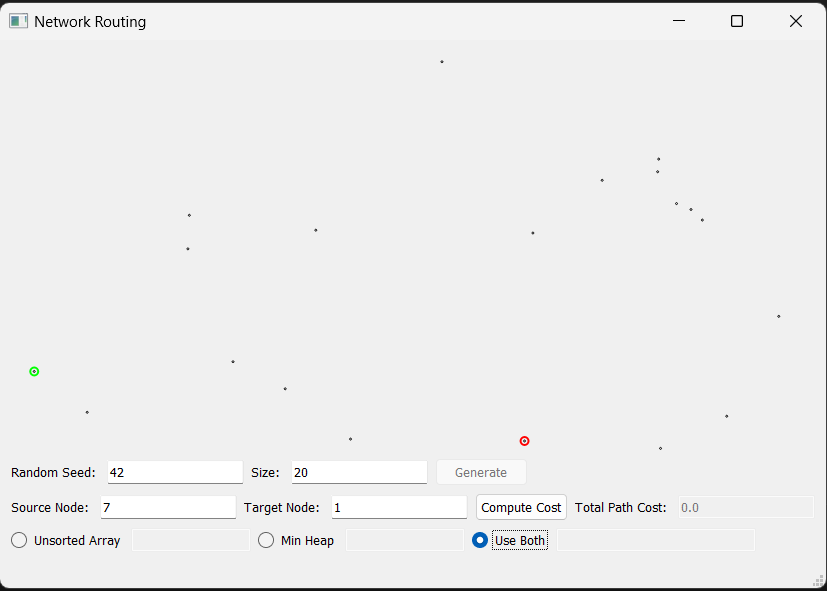
\includegraphics[width=0.80\linewidth]{figures/42.png} 
      \caption{For Random seed 42 - Size 20, use node 7 (the left-most node) as the source and node 1 (on the bottom toward the right) as the destination}\label{fig:42}
    \end{center}
  \end{figure}

\noindent The figure (in figure 2) shows the 20 sample generated using seed 42. The source node is 7 and the target node is 1. But the target was unreachable from the given source. Thus, I could not include the time taken by the program and conclude that the target is unreachable. 
\newpage

\begin{figure}[h]. % the 't' asks LaTeX to put this figure on the top of the page   
    \begin{center}
      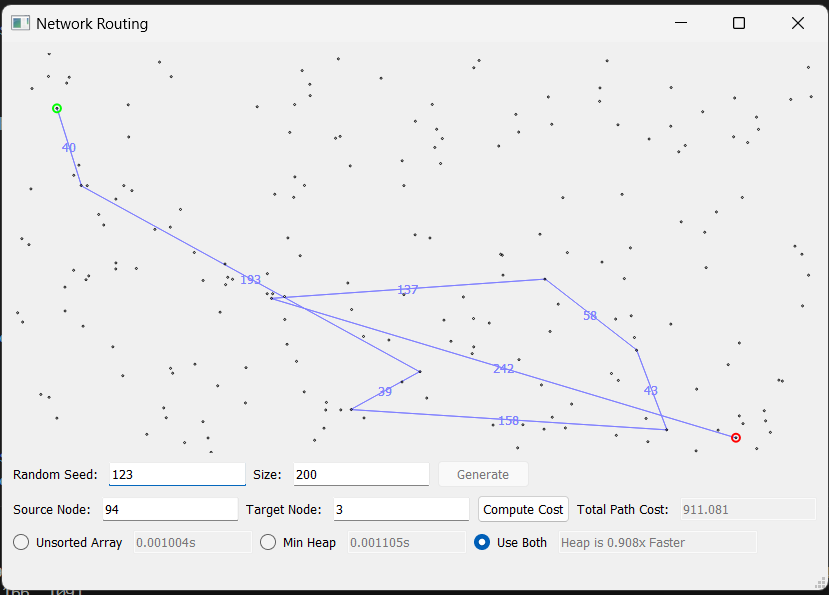
\includegraphics[width=0.80\linewidth]{figures/943.png} 
      \caption{For Random seed 123 - Size 200, use node 94 (near the upper left) as the source and node 3 (near the lower right) as the destination}\label{fig:943}
    \end{center}
  \end{figure}

\noindent The figure (in figure 3) shows the 200 sample generated using seed 123. The source node is 94 and the target node is 3. The total time taken to compute the Dijkstra’s algorithm using array is 0.00100 sec and for binary heap it took 0.001105 sec i.e. the heap is 0.908 times faster. And the total cost of tree is 911.081.

\newpage

\begin{figure}[h]. % the 't' asks LaTeX to put this figure on the top of the page   
    \begin{center}
      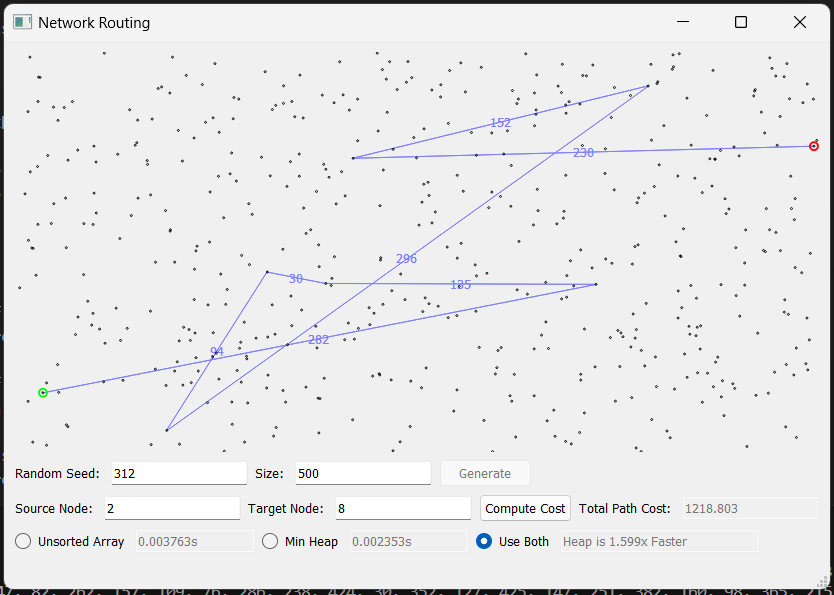
\includegraphics[width=0.80\linewidth]{figures/28.png} 
      \caption{For Random seed 312 - Size 500, use node 2 (near the lower left) as the source and node 8 (near the upper right) as the destination}\label{fig:28}
    \end{center}
  \end{figure}

\noindent The figure (in figure 4) shows the 500 sample generated using seed 312. The source node is 2 and the target node is 8. The total time taken to compute the Dijkstra’s algorithm using array is 0.0.00376 sec and for binary heap it took 0.0.00235 sec i.e. the heap is 1.5999 times faster. And the total cost of tree is 1218.803.

\newpage

\section{Conclusion}
I was able to generate the code to compute the Dijkstra’s algorithm using the array and binary priority queue. I was able to estimate the time taken to compute the sample size of 1000000 for array queue. Also, I have analyzed the time complexity of both the priority queue. 


\end{document}